% Created 2022-09-10 sáb 16:23
% Intended LaTeX compiler: pdflatex
\documentclass[12pt]{article}
\usepackage[utf8]{inputenc}
\usepackage[T1]{fontenc}
\usepackage{graphicx}
\usepackage{grffile}
\usepackage{longtable}
\usepackage{wrapfig}
\usepackage{rotating}
\usepackage[normalem]{ulem}
\usepackage{amsmath}
\usepackage{textcomp}
\usepackage{amssymb}
\usepackage{capt-of}
\usepackage{hyperref}
\usepackage[spanish]{babel}
\usepackage{graphicx,geometry}
\geometry{ a4paper, left=1in, right=1in, top=1in, bottom=1in }
\renewcommand\familydefault{\sfdefault}
\usepackage{sectsty}
\sectionfont{\normalfont\large }
\usepackage{tabularx}
\usepackage{listings}
\lstdefinestyle{mystyle}{
numbers=left,
showspaces=false,
frame=leftline,
showspaces=false,
showstringspaces=false,
showtabs=false,
numberstyle=\tiny,
}
\lstset{
style=mystyle,
literate={á}{{\'a}}1
{é}{{\'e}}1
{í}{{\'{\i}}}1
{ó}{{\'o}}1
{ú}{{\'u}}1
{Á}{{\'A}}1
{É}{{\'E}}1
{Í}{{\'I}}1
{Ó}{{\'O}}1
{Ú}{{\'U}}1
{ü}{{\"u}}1
{Ü}{{\"U}}1
{ñ}{{\~n}}1
{Ñ}{{\~N}}1
{¿}{{?``}}1
{¡}{{!``}}1
}
\makeatletter
\usepackage{fancyhdr}
\pagestyle{fancy}
\usepackage{mdframed}
\BeforeBeginEnvironment{minted}{\begin{mdframed}}
\AfterEndEnvironment{minted}{\end{mdframed}}
\author{Luis Eduardo Galindo Amaya (1274895)}
\date{2022-09-10}
\title{Exploración de marcos de trabajo.}
\hypersetup{
 pdfauthor={Luis Eduardo Galindo Amaya (1274895)},
 pdftitle={Exploración de marcos de trabajo.},
 pdfkeywords={},
 pdfsubject={},
 pdfcreator={Emacs 26.3 (Org mode 9.1.9)}, 
 pdflang={Spanish}}
\begin{document}


\newcommand{\docente}{Manuel Castañón-Puga}
\newcommand{\asignatura}{Herramientas de Desarrollo de Software (40017)}
\newcommand{\semestre}{2022-2}

\newcommand{\miportada}[1]{
	\begin{titlepage}
		\vspace*{0.75in}
		\begin{flushleft}
			\sffamily
			\large #1       \\
			\Huge 
            \@title         \\
			\hrulefill
			\vspace{0.25in} \\
			\Large \@author \\
			\vspace*{\fill}
            
\includegraphics[width=\textwidth]{../includes/filler.png} \\
			\vspace*{\fill}
			\large
			\begin{tabular}{|l|l|}
              \hline
			  Asignatura & \asignatura \\
			  Docente    & \docente    \\
			  Fecha      & \@date      \\
              \hline
			\end{tabular}
		\end{flushleft}
	\end{titlepage}
}

\fancyhf{}
\lhead{ \asignatura }
\rhead{ \semestre }
\rfoot{Página \thepage}

\setlength\parindent{0pt}   % eliminar el intentado
\setlength{\parskip}{1.2em}
% \maketitle

\thispagestyle{empty}
\begin{center}
	{\large
		UNIVERSIDAD AUTÓNOMA DE BAJA CALIFORNIA \\
		Facultad de Ciencias Químicas e Ingeniería }
	\vspace{0.25in} \\
	Programa de Ingeniero en Software y Tecnologías Emergentes
\end{center}

\section*{Información De La Materia}
\label{sec:org41b86f6}
\begin{mdframed}
\begin{description}
\item[{Asignatura}] \asignatura .
\item[{Grupo y Periodo}] 341 (2022-2) .
\item[{Docente}] \docente .
\end{description}
\end{mdframed}

\section*{Información De La Actividad}
\label{sec:org1dab59f}
\begin{mdframed}
\begin{description}
\item[{Nombre de la actividad}] Exploración de marcos de trabajo.
\item[{Fecha}] 2022-09-10
\item[{Lugar}] Edificio 6E, Salón 204.
\item[{Carácter de la actividad}] Individual.
\item[{Participante(es)}] Luis Eduardo Galindo Amaya (1274895).
\end{description}
\end{mdframed}

\section*{Reporte De Actividades}
\label{sec:org2c77552}
\subsection*{Spring}
\label{sec:org8829f4a}
Fue la mas tardada en usar pero sin duda es la que se siente mas robusta de las cuatro, el paradigma de java funciona muy bien con este tipo de aplicaciones web.

\begin{center}
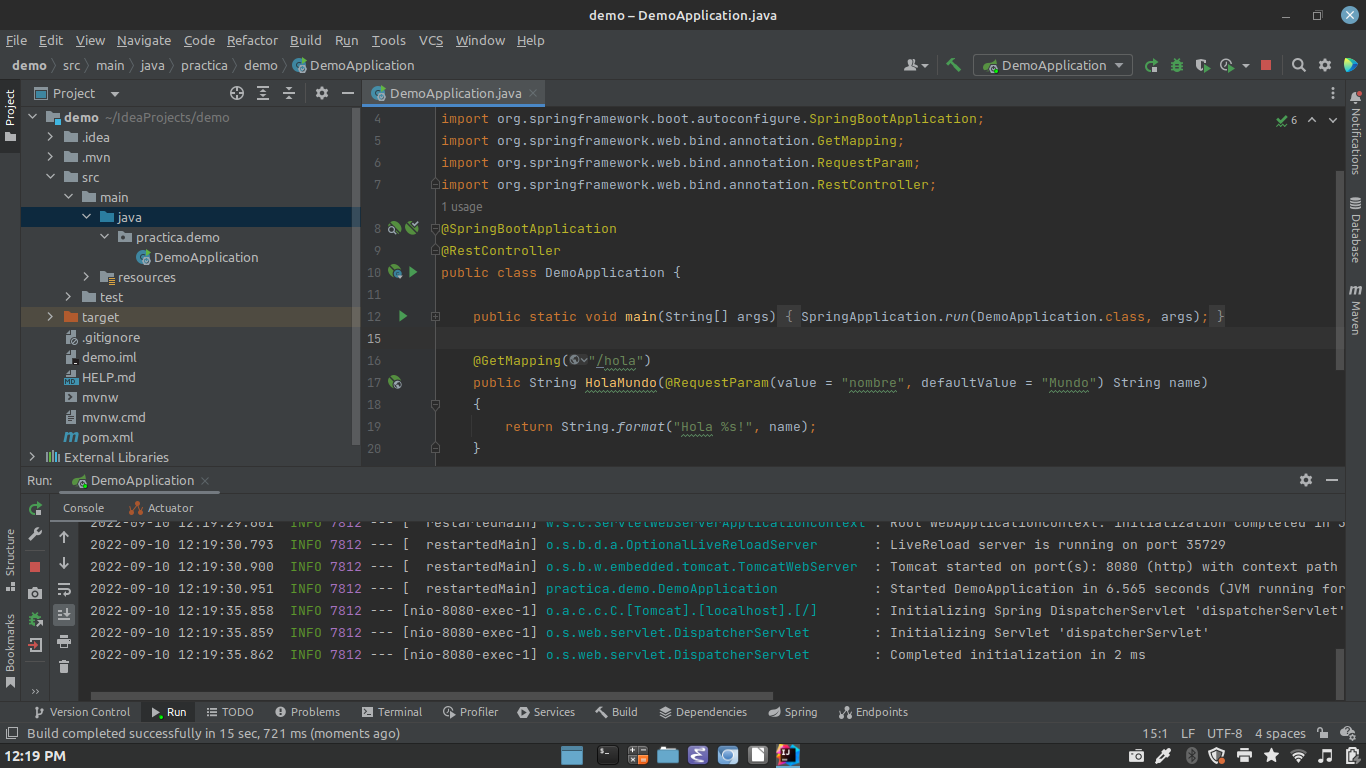
\includegraphics[width=.9\linewidth]{img/Spring-codigo.png}
\end{center}

\begin{center}
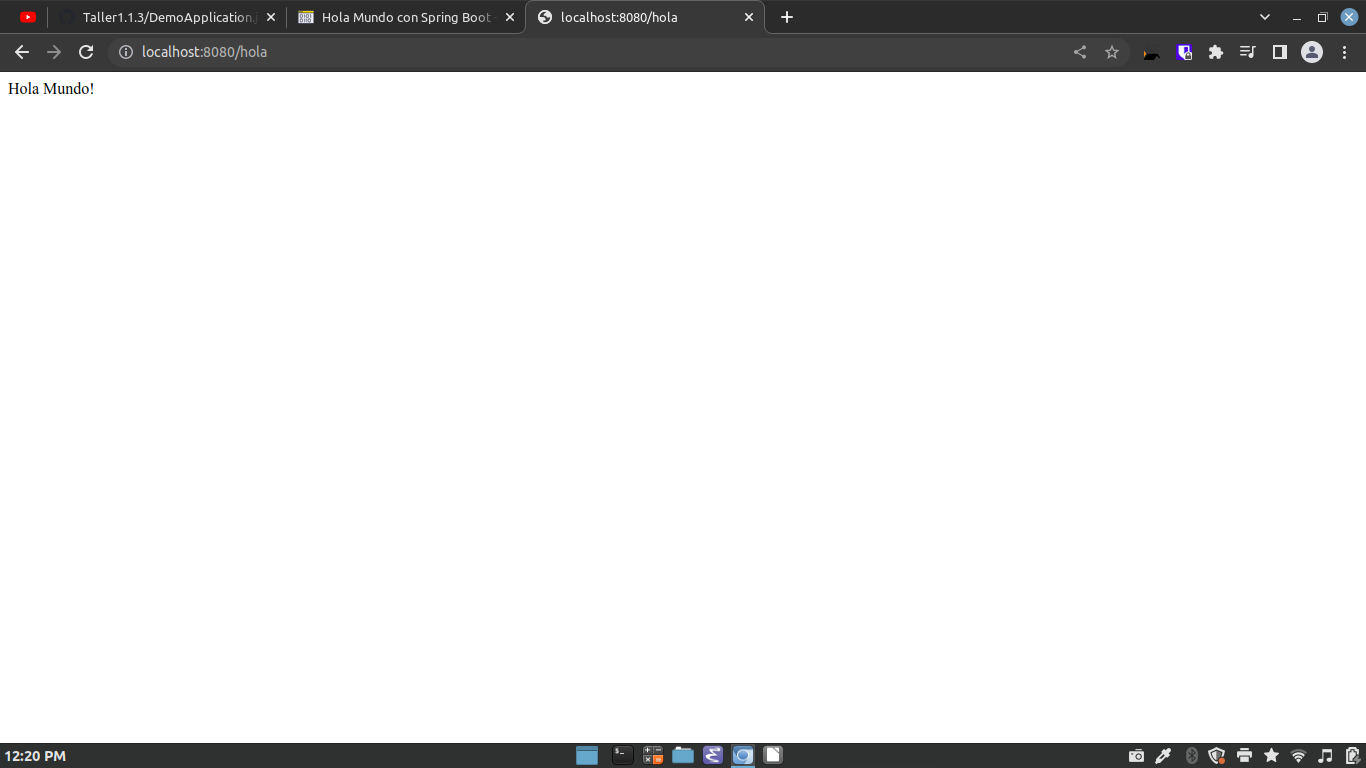
\includegraphics[width=.9\linewidth]{img/Spring-navegador.png}
\end{center}

\begin{center}
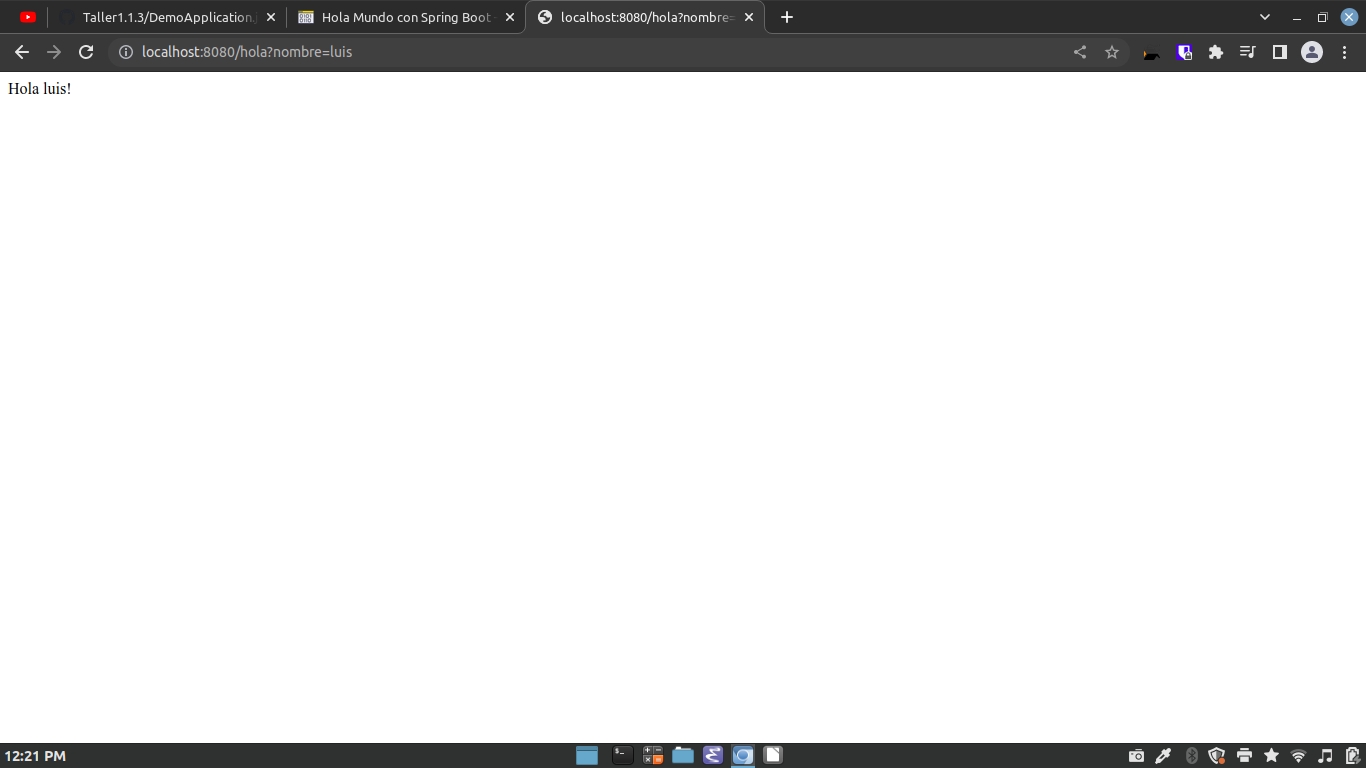
\includegraphics[width=.9\linewidth]{img/Spring-parametro.png}
\end{center}

\subsection*{JavaFx}
\label{sec:org9558c5f}
Este es otro paquete para hacer GUIs en java, tenemos AWT y swing pero javafx se siente mas pulido que los últimos dos, tomando en cuenta que su forma de estilar las aplicaciones es por medio de css se siente mucho mas atemporal que swing pero es muchísimo mas demandante. 

\begin{center}
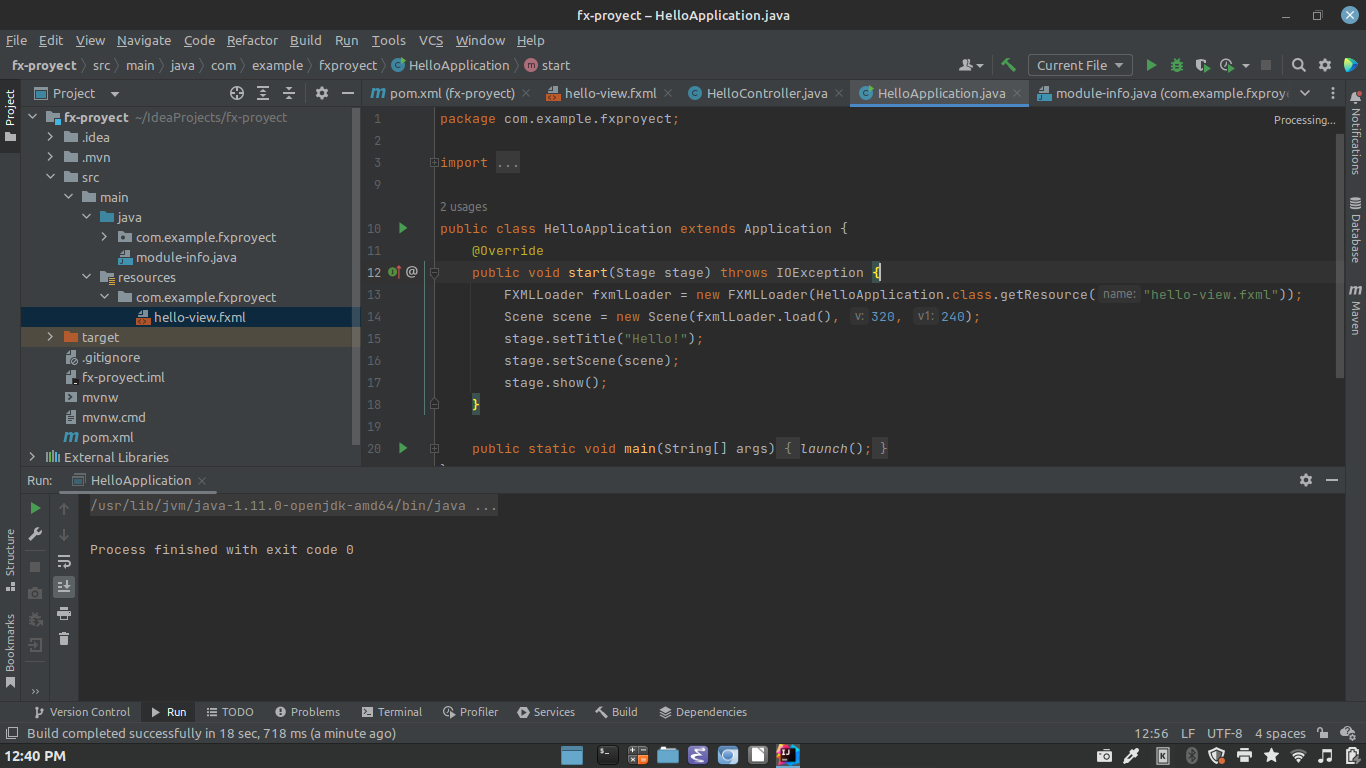
\includegraphics[width=.9\linewidth]{img/fx-code.png}
\end{center}

\begin{center}
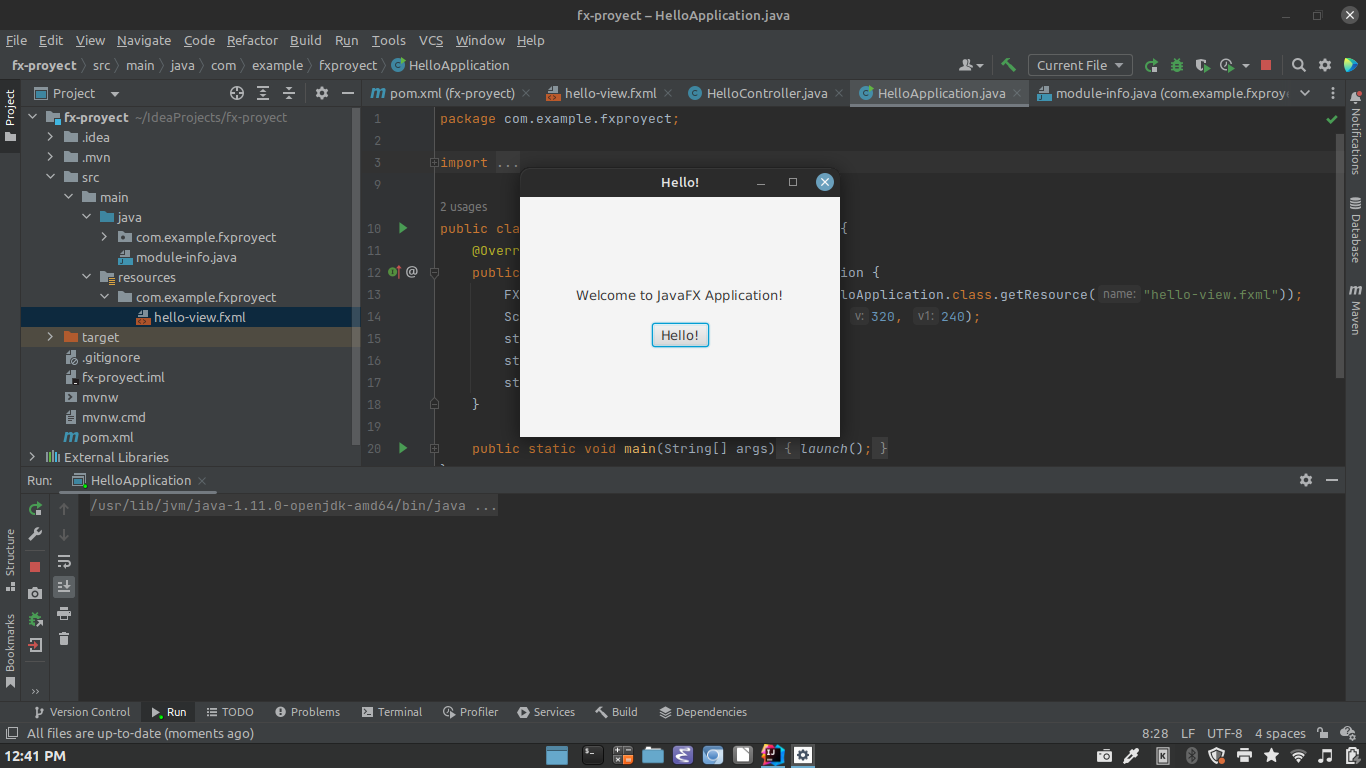
\includegraphics[width=.9\linewidth]{img/fx-out.png}
\end{center}

\subsection*{Django}
\label{sec:orga70b640}
Crear aplicaciones web en Django es muchísimo mas sencillo que en Spring, puede ser que sea menos robusto pero es mas fácil de montar un proyecto y lanzarlo pronto en Django que en Spring. 

\begin{center}
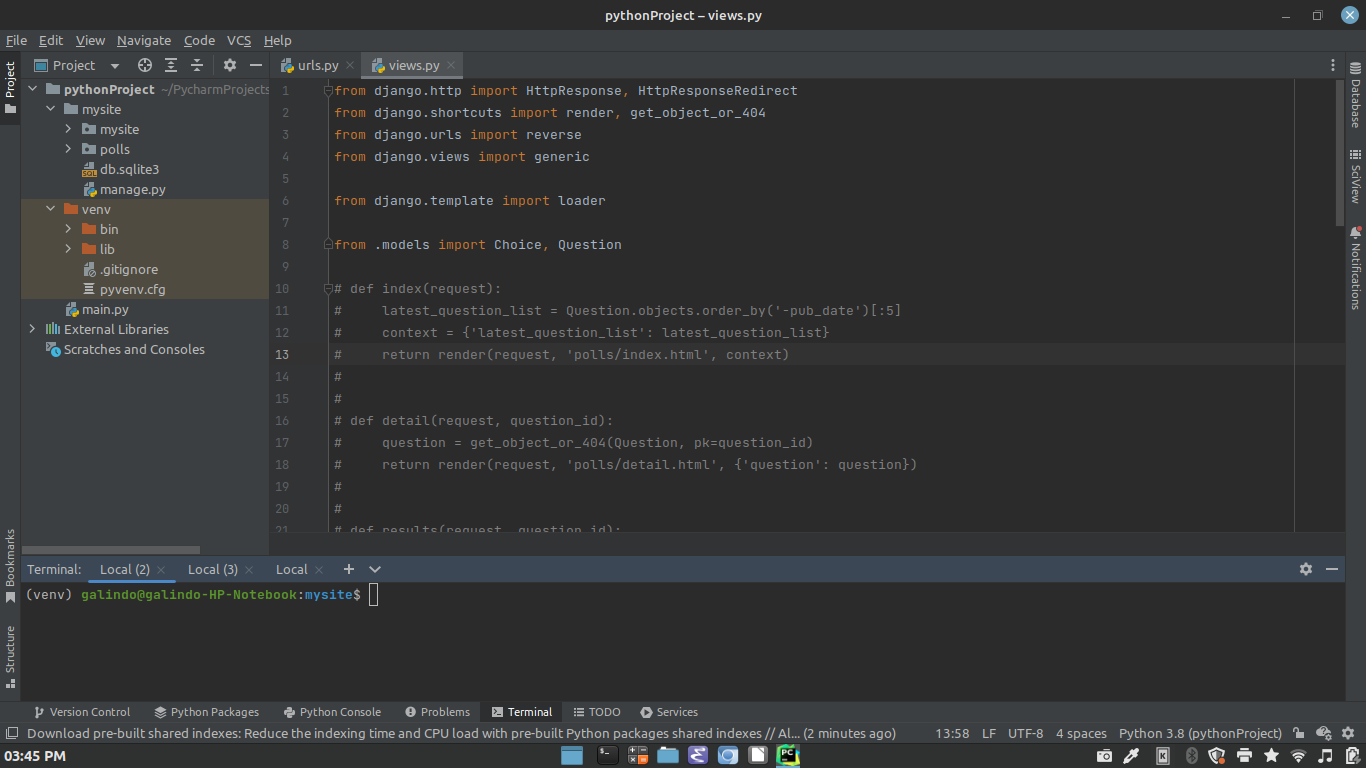
\includegraphics[width=.9\linewidth]{img/django-code.png}
\end{center}

\begin{center}
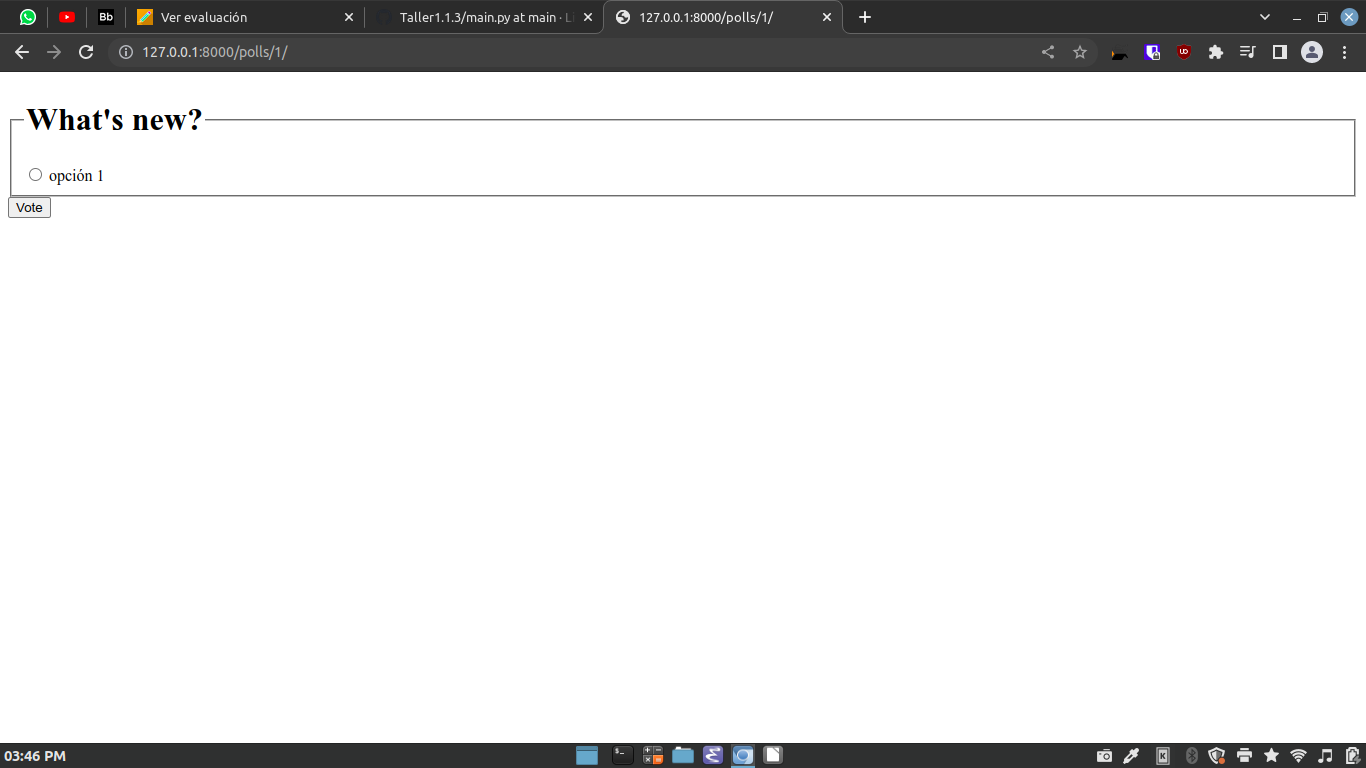
\includegraphics[width=.9\linewidth]{img/django-polls.png}
\end{center}

\subsection*{tktinker}
\label{sec:org3c795b9}
Es un paquete para crear GUIs en python, nada destacable mas que su facilidad de uso pero puede ayudarnos a crear una aplicacion multiplataforma mas facilmente.

\begin{center}
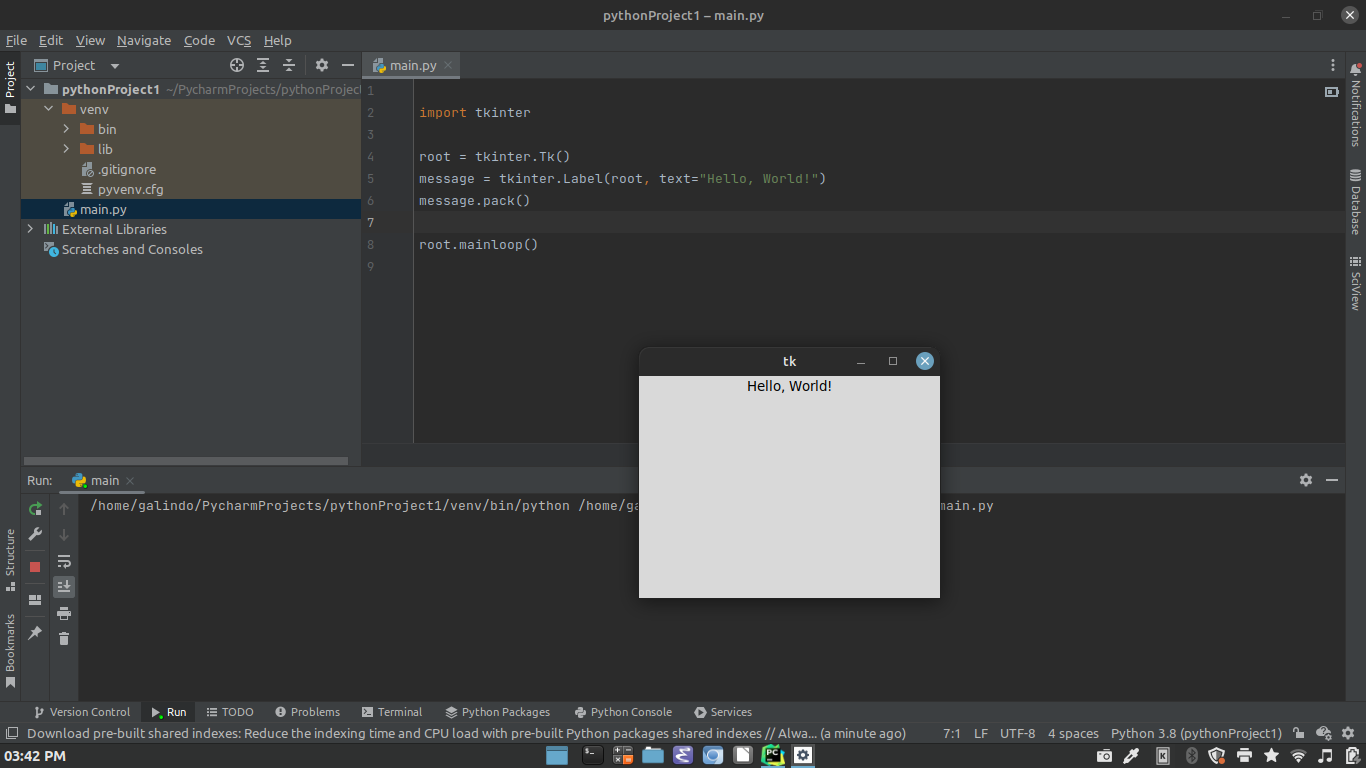
\includegraphics[width=.9\linewidth]{img/tk.png}
\end{center}


\section*{Reflexión}
\label{sec:org74dd750}
\begin{mdframed}
Las herramientas que revisamos son muy interesantes a que reflejan los dos modos de operacion para el ususario as comunes, por medio del navegador y por medio de una GUI, tradicionalmente usamos interfaces de terminal para hacer nuestros proyectos pero en nuestro dia a dia (normalmente) no solemos usarlas y que es mas sencillo usar las herramientas en un medio grafico. 
\end{mdframed}

\begin{center}
Doy fe de que toda la información dada es  completa y correcta. \\
\begin{center}

\includegraphics[width=3cm]{../includes/firma.png}
\end{center}
Luis Eduardo Galindo Amaya (1274895)
\end{center}
\end{document}
